% Fragmento: Fase 0 — Fundamentos reproducibles y datos
% Tareas asignadas: TASK-1, TASK-2, TASK-3, TASK-4, TASK-5, TASK-6
% Plantilla: ver sección «Propósito y convenciones» de la bitácora.
% Obligatorio: \label{hallazgo:task-N} por cada tarea documentada.

\subsubsection{Task-1: Infraestructura y entorno reproducible}
\label{hallazgo:task-1}
\begin{tabularx}{\textwidth}{|l|X|}\hline
\textbf{Fecha} & 2026-08-16 \\\hline
\textbf{Actividad} & Infraestructura (m-0) \\\hline
\textbf{Artefactos} & \texttt{src/config.py}, \texttt{src/utils/seed.py}, \texttt{src/utils/device.py}, \texttt{src/smoke.py}, \texttt{uv.lock}, \texttt{.python-version} \\\hline
\end{tabularx}

\paragraph{Objetivo.}
Establecer un entorno reproducible con una única fuente de hiperparámetros,
semilla global fijada y selección de dispositivo \texttt{cuda > mps > cpu}.

\paragraph{Procedimiento.}
Se implementó \texttt{ExperimentConfig} como dataclass congelada, \texttt{set\_seed(42)}
con \texttt{torch.use\_deterministic\_algorithms(True, warn\_only=True)} y
\texttt{get\_device()} con la prelación definida en \texttt{AGENTS.md}.
Verificación con:
\begin{verbatim}
uv run python -m src.smoke
\end{verbatim}

\paragraph{Resultados.}
Stack congelado: Python 3.12, PyTorch 2.9.1, torchvision 0.24.1,
PennyLane 0.45.1, NumPy $\geq 2.0,< 2.3$.
Dispositivo detectado: \textbf{mps}.
Pérdida de referencia (dos corridas idénticas): \textbf{1.54205954}.
Resultado reproducibilidad: \textbf{PASS}.

\paragraph{Interpretación.}
El entorno local cumple el criterio de reproducibilidad bit a bit dentro del mismo
dispositivo. La semilla 42 queda fijada por convención del anteproyecto.

\paragraph{Decisiones.}
Semilla global 42 en \texttt{ExperimentConfig.semilla}.
Gestor de paquetes exclusivo: UV (\texttt{uv sync --frozen}).
Dispositivo registrado en cada corrida (contrato de tarea 4).

\paragraph{Limitaciones.}
La reproducibilidad bit a bit solo se garantiza dentro del mismo dispositivo;
en \texttt{mps} algunas operaciones caen a CPU sin equivalente completo de
\texttt{torch.cuda.manual\_seed\_all}.

\subsubsection{Task-2: Estructura LaTeX del trabajo de grado y bitácora de hallazgos}
\label{hallazgo:task-2}
\begin{tabularx}{\textwidth}{|l|X|}\hline
\textbf{Fecha} & 2026-08-16 \\\hline
\textbf{Actividad} & Documentación (m-0) \\\hline
\textbf{Artefactos} & \texttt{docs/trabajo\_de\_grado/} (bitácora, preámbulo, esqueleto de tesis, fragmentos \texttt{hallazgos/}) \\\hline
\end{tabularx}

\paragraph{Objetivo.}
Crear la estructura LaTeX del documento final y la bitácora metodológica de hallazgos,
con trazabilidad \texttt{task-N} $\leftrightarrow$ artefactos en \texttt{results/}.

\paragraph{Procedimiento.}
Se copió el preámbulo UAO del anteproyecto a \texttt{preambulo\_uao.tex} sin modificar
el original. Se crearon los fragmentos \texttt{h0\_fundamentos.tex} a \texttt{h3\_analisis.tex},
el esqueleto \texttt{Trabajo de Grado - Frank Daza.tex} con capítulos vacíos y la cadena
de compilación \texttt{pdflatex} $\rightarrow$ \texttt{bibtex} $\rightarrow$ \texttt{pdflatex}
contra \texttt{../proyecto\_de\_grado/Referencias.bib}.

\paragraph{Resultados.}
Estructura creada en \texttt{docs/trabajo\_de\_grado/}:
\texttt{preambulo\_uao.tex}, bitácora, esqueleto de tesis, carpetas \texttt{hallazgos/},
\texttt{capitulos/} y \texttt{Figuras/} (logo UAO).
Bibliografía compartida sin entradas duplicadas.
Cita de verificación: PennyLane~\cite{bergholm2018pennylane}.

\paragraph{Interpretación.}
A partir de esta tarea, cada hallazgo experimental se registra en el fragmento de fase
correspondiente. El documento final (tarea 17) sintetizará esta evidencia con
\texttt{\textbackslash ref\{hallazgo:task-N\}} en lugar de reconstruir resultados desde CSV.

\paragraph{Decisiones.}
Preámbulo copiado (no refactorizado) del anteproyecto entregado.
Fragmentos sin espacios en el nombre de archivo.
Logo UAO copiado (no symlink) para portabilidad entre máquinas.

\paragraph{Limitaciones.}
Los documentos principales (\texttt{Bitacora Metodologica de Hallazgos.tex},
\texttt{Trabajo de Grado - Frank Daza.tex}) llevan espacios en el nombre;
la compilación requiere comillas en la línea de comandos.

\subsubsection{Task-3: Auditoría del Brain Tumor MRI Dataset (A4)}
\label{hallazgo:task-3}
\begin{tabularx}{\textwidth}{|l|X|}\hline
\textbf{Fecha} & 2026-08-17 \\\hline
\textbf{Actividad} & A4 --- Curaduría y auditoría del dataset (m-0) \\\hline
\textbf{Artefactos} & \texttt{src/data/audit.py}, \texttt{results/dataset\_manifest.csv}, \texttt{results/dataset\_audit.md}, \texttt{results/figures/distribucion\_clases.png} \\\hline
\end{tabularx}

\paragraph{Objetivo.}
Verificar el conteo real, el balance por clase y partición, la integridad de las
imágenes y la presencia de duplicados exactos antes de diseñar escenarios de
escasez, siguiendo buenas prácticas de preparación de datos en imagen médica~\cite{willemink2020preparing}.

\paragraph{Procedimiento.}
Dataset local en \texttt{notebooks/data/}, enlazado por symlink a
\texttt{data/brain\_tumor\_mri/} (ruta de \texttt{ExperimentConfig}).
Recorrido estable con \texttt{pathlib}, verificación PIL (\texttt{verify} +
\texttt{load}), hash SHA-256 de contenido y clasificación de duplicados en tres
categorías. Ejecución:
\begin{verbatim}
uv run python -m src.data.audit
\end{verbatim}

\paragraph{Resultados.}
Total inventariado: \textbf{7023} imágenes (coincide con el anteproyecto).
Extensiones: solo \texttt{.jpg}. Imágenes corruptas: \textbf{0}.
Duplicados exactos (grupos con $n>1$): intra clase \textbf{194}, entre clases
\textbf{0}, Training$\leftrightarrow$Testing \textbf{79}.
Exclusiones: \textbf{297} filas (\texttt{duplicado\_exacto}: 194;
\texttt{fuga\_train\_test}: 103). Utilizables: \textbf{6726}.

\begin{center}
\begin{tabular}{lrrrr}\hline
\textbf{Clase} & \textbf{Testing} & \textbf{Training} & \textbf{Total} \\\hline
glioma       & 300 & 1321 & 1621 \\
meningioma   & 306 & 1339 & 1645 \\
notumor      & 405 & 1595 & 2000 \\
pituitary    & 300 & 1457 & 1757 \\\hline
\textbf{Total} & 1311 & 5712 & 7023 \\\hline
\end{tabular}
\end{center}

Heterogeneidad: modos \texttt{L} (3093), \texttt{RGB} (3926), \texttt{P}/\texttt{RGBA} (4);
resolución dominante $512\times512$ (4742 imágenes). Las cuatro clases corresponden
a categorías del sistema nervioso central en la clasificación WHO 2021~\cite{louis20212021}.

\begin{figure}[ht]
\centering
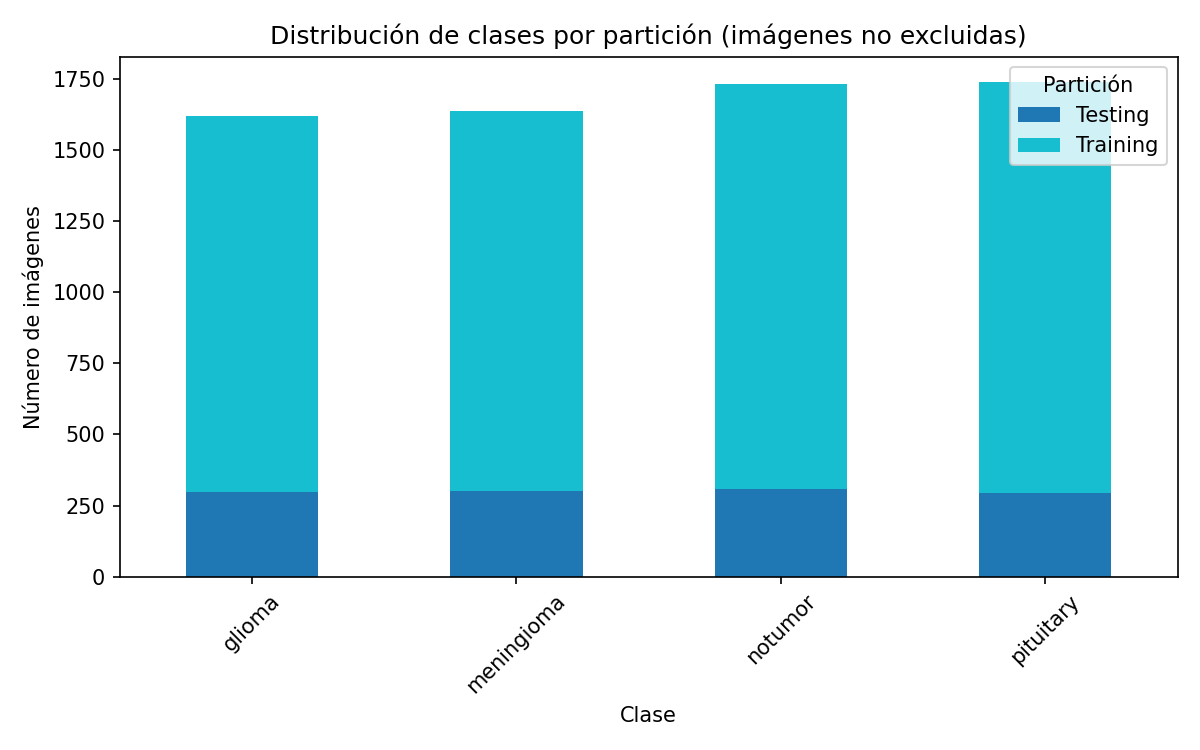
\includegraphics[width=0.85\textwidth]{../../../results/figures/distribucion_clases}
\caption{Distribución de clases por partición (imágenes no excluidas).}
\label{fig:distribucion-clases-task3}
\end{figure}

\paragraph{Interpretación.}
El dataset agregado de Nickparvar~\cite{nickparvar2023dataset} es heterogéneo en
modo de color y resolución; la auditoría confirma que el tamaño declarado es correcto
pero existen duplicados exactos y fuga potencial entre \texttt{Training/} y
\texttt{Testing/}. Sin esta verificación, la exactitud de modelos posteriores
podría inflarse por memorización de copias idénticas~\cite{haddou2025hqcm}.

\paragraph{Decisiones.}
Unir \texttt{Training/} y \texttt{Testing/} al conjunto completo para validación
cruzada estratificada $k=5$ (decisión D1, TASK-6); no se usa \texttt{Testing/} como
holdout externo. Las exclusiones quedan en \texttt{dataset\_manifest.csv} mediante
columnas \texttt{excluida} y \texttt{motivo\_exclusion}.

\paragraph{Limitaciones.}
El hash SHA-256 detecta duplicados byte a byte, no re-codificaciones JPEG con distinta
compresión. La conversión a 3 canales y el redimensionado a $224\times224$ quedan
para TASK-5.

% --- Tareas pendientes en este fragmento ---
% TASK-4: Contrato de métricas, logging y artefactos
% TASK-5: Pipeline de preprocesamiento y aumento de datos (A5)
% TASK-6: Protocolo de particiones: holdout, k-fold y fracciones (A7)
